\documentclass[a4paper,12pt]{article} % тип документа

% Поля страниц
\usepackage[left=2.5cm,right=2.5cm, top=2cm,bottom=2cm,bindingoffset=0cm]{geometry}

%Пакет дял таблиц   
\usepackage{multirow} 

%Отступ после заголовка    
\usepackage{indentfirst}


% Рисунки
\usepackage{subcaption,floatrow,graphicx,calc}
\usepackage{wrapfig}

% Создаёем новый разделитель
\DeclareFloatSeparators{mysep}{\hspace{1cm}}

% Ссылки?
\usepackage{hyperref}
\usepackage[rgb]{xcolor}
\hypersetup{				% Гиперссылки
	colorlinks=true,       	% false: ссылки в рамках
	urlcolor=blue          % на URL
}


%  Русский язык
\usepackage[T2A]{fontenc}			% кодировка
\usepackage[utf8]{inputenc}			% кодировка исходного текста
\usepackage[english,russian]{babel}	% локализация и переносы


% Математика
\usepackage{amsmath,amsfonts,amssymb,amsthm,mathtools, mathrsfs, wasysym}

\author{Гаврилин Илья\\
		Добровольская Ксения\\
	Б01-110}
\title{\textbf{Лабораторная работа 4.2\\ 
		 Изучение энергетического спектра $\beta$-частиц и определение их максимальной энергии при помощи магнитного спектрометра}}
\begin{document}
	\maketitle
	\textbf{Цель работы:} с помощью магнитного спектрометра исследовать энергетический спектр $\beta$-частиц при распаде ядер $^{137}$Cs и определить их максимальную энергию.
	\textbf{Оборудование:} Источник $\beta$ частиц ($^{137}$Cs), система фокусировки и отделения частиц ("магнитная линза"), вакуумный насос и вакуумметр, компьютеризированный счетчик частиц.
	
	\section{Теоретическая часть}
	
	Бета-распад - самопроизвольное превращение ядер, при котором их массовое число не изменяется, а заряд увеличивается или уменьшается на единицу.
	В данной работе:
	$$^A_Z X \to ^{\ \, A}_{Z+1} X + e^- + \widetilde{\nu} .$$
	
	Величина $W(p_e)$ является плотностью вероятности. Распределение электронов по энергии может быть вычислено теоретически. Для разрешенных переходов вероятность $\beta$-распада просто пропорциональна статистическому весу.
	\begin{equation*}
		\label{eq:W}
		W(p_e)dp_e \propto p_e^2(E_m-E_e)^2 dp_e.
	\end{equation*}
	Кинетическая энергия электрона и его импульс связаны друг с другом обычной формулой:
	\begin{equation*}
		E = \sqrt{(p_ec)^2+(m_ec^2)^2}-m_ec^2
	\end{equation*}
	Выражение (\ref{eq:W}) приводит к спектру, имеющему вид широкого колокола. Кривая плавно отходит от нулся и стольже плавно, по параболе, касается оси абсцисс в области максимального импульса электронов.
	
	Дочерние ядра, возникающие в результате $\beta$-распада, нередко оказываются возбужденными. Возбужденные ядра отдают свою энергию либо излучая $\gamma$-квант, либо передвавая избыток энергии одному из электронов внутренних оболочек атома. Излучаемые в таком процессе электроны имеют строго определенную энергию и называются \textit{конверсионными}.
	
	Конверсия чаще всего происходит на оболочках K и L. Ширина конверсионной линии является чисто аппаратурной -- по ней можно оценить разрешающую силу спектрометра.
	
	\section{Экспериментальная установка}
	Блок-схема установки для изучения $\beta$-спектров изображена на рис. \ref{pic1}. Радиоактивный источник $^{137}$Cs помещен внутрь откачанной трубы. Электроны, сфокусированные магнитной линзой, попадают в счетчик. В газоразрядном счетчике они инициируют газовый разряд и тем самым приводят к появлению электрических импульсов на электродах, которые затем регистрируются пересчетным прибором.
	
	
	\thisfloatsetup{floatrowsep=mysep}	
	\begin{figure}[h!]
		\ffigbox{
			\begin{subfloatrow}[2]
				\ffigbox[\FBwidth]{\caption{}}%
				{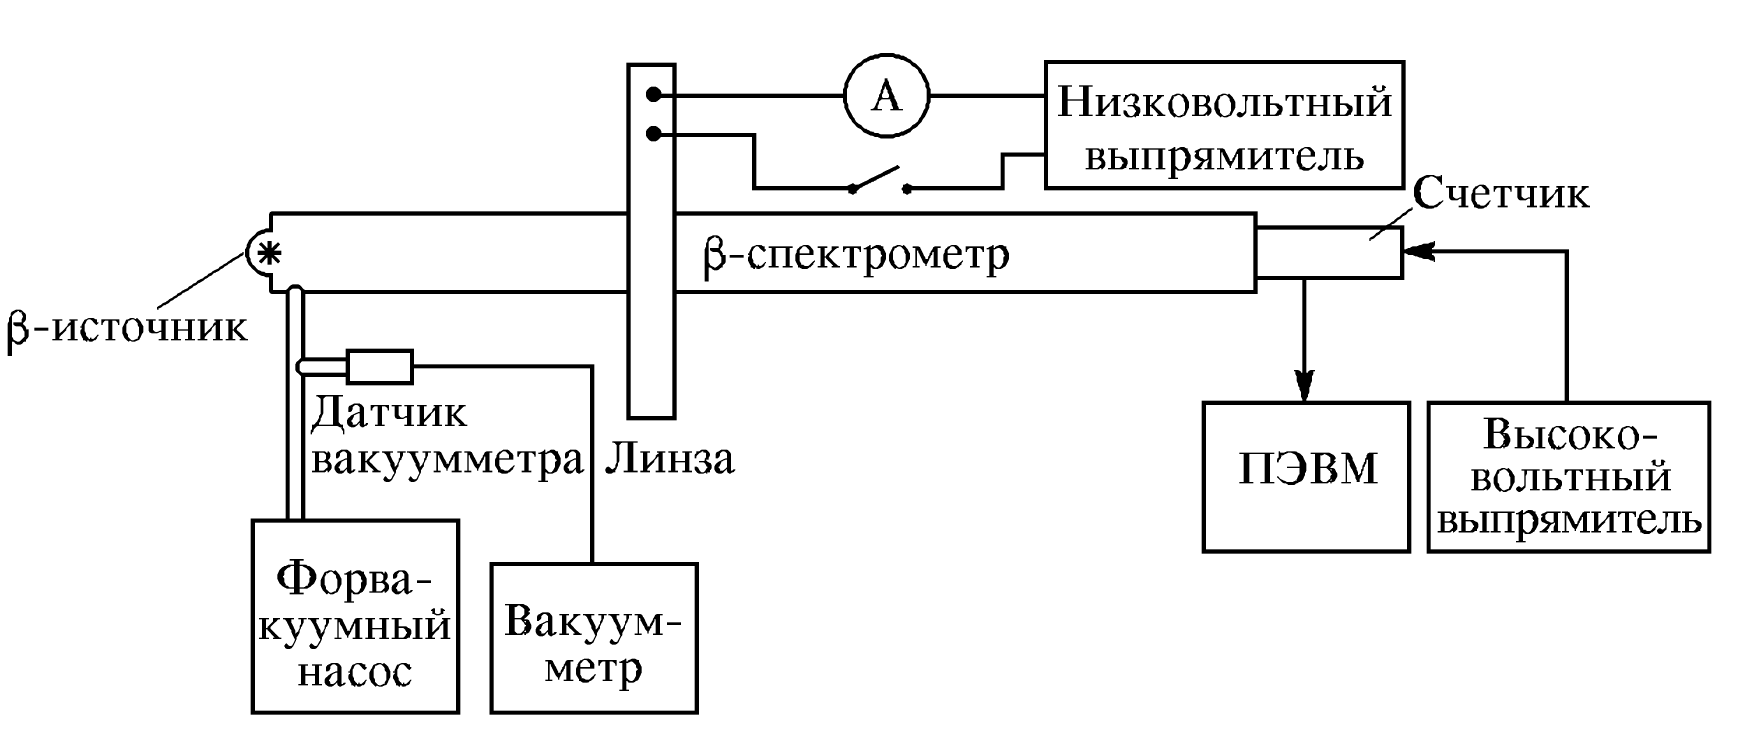
\includegraphics[width=8cm,height=4cm]{shema.png}{\label{pic1}}}
				\ffigbox[\FBwidth]{\caption{}}%
				{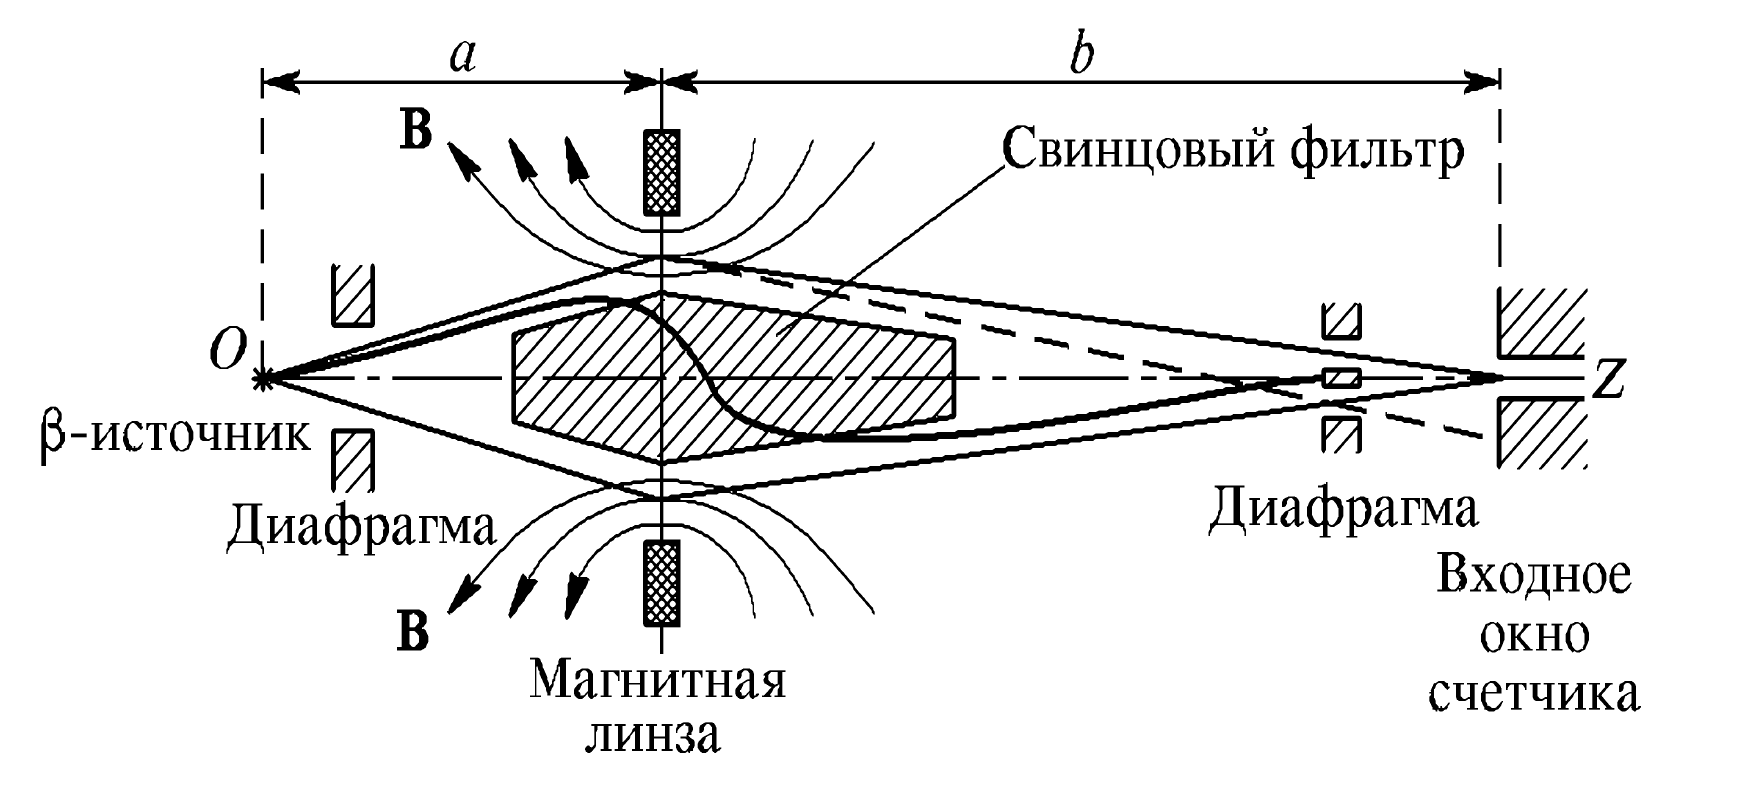
\includegraphics[width=8cm,height=4cm]{ustanovka.png}{\label{pic2}}}         
			\end{subfloatrow}
		}
		{\caption{Экспериментальная установка.}}
	\end{figure}
	
	Энергию $\beta$-частиц определяют с помощью $\beta$-спектрометров (рис.~\ref{pic2}). В работе используется магнитный спектрометр с <<короткой линзой>>. Отметим, что в течение всего опыта геометрия прибора остается неизменной, поэтому импульс сфокусированных электронов пропорционален величине тока:
	\begin{equation}
		\label{eq:pkI}
		\tag{$\star$}
		p_e = kI.
	\end{equation}
	
	Cвязь между числом частиц, регистрируемых установкой, и функцией $W(p_e)$ выражается формулой:
	\begin{equation*}
		N(p_e) \propto W(p_e)p_e,
	\end{equation*}
	откуда
	\begin{equation}
		\label{eq:fermi}
		\tag{$\star \star$}
		\frac{\sqrt{N}}{p_e^{3/2}} \propto E_m - E
	\end{equation}
	
	
	\section{Ход работы}
	1. Подготовим установку к работе: откачаем воздух, включим формирователь импульсов, счетчик, магнитную линзу.\\
	2. Когда давление по вакуумметру станет достаточно низким начнем производить замеры.\\
	3. Подробно замерим излучение при различных значениях тока, подробно постараемся замерить конверсионный пик.
	\begin{figure}[H]
		\centering
		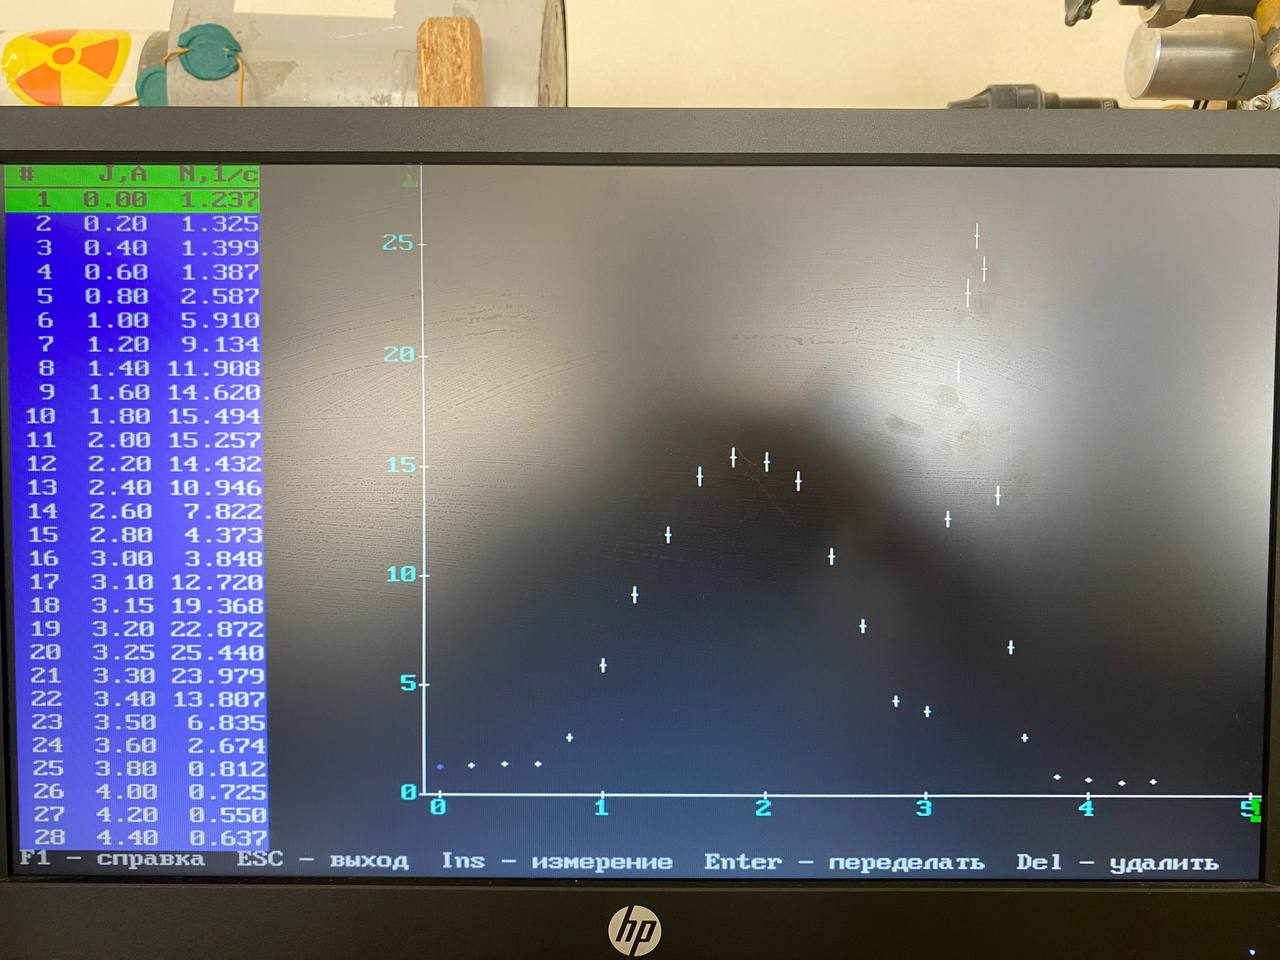
\includegraphics[width=0.7\linewidth]{pc_1}
		\caption{график зависимости числа $\beta$ распадов от тока в катушке без учета фона}
		\label{fig:pc1}
	\end{figure}
	\begin{figure}[H]
		\centering
		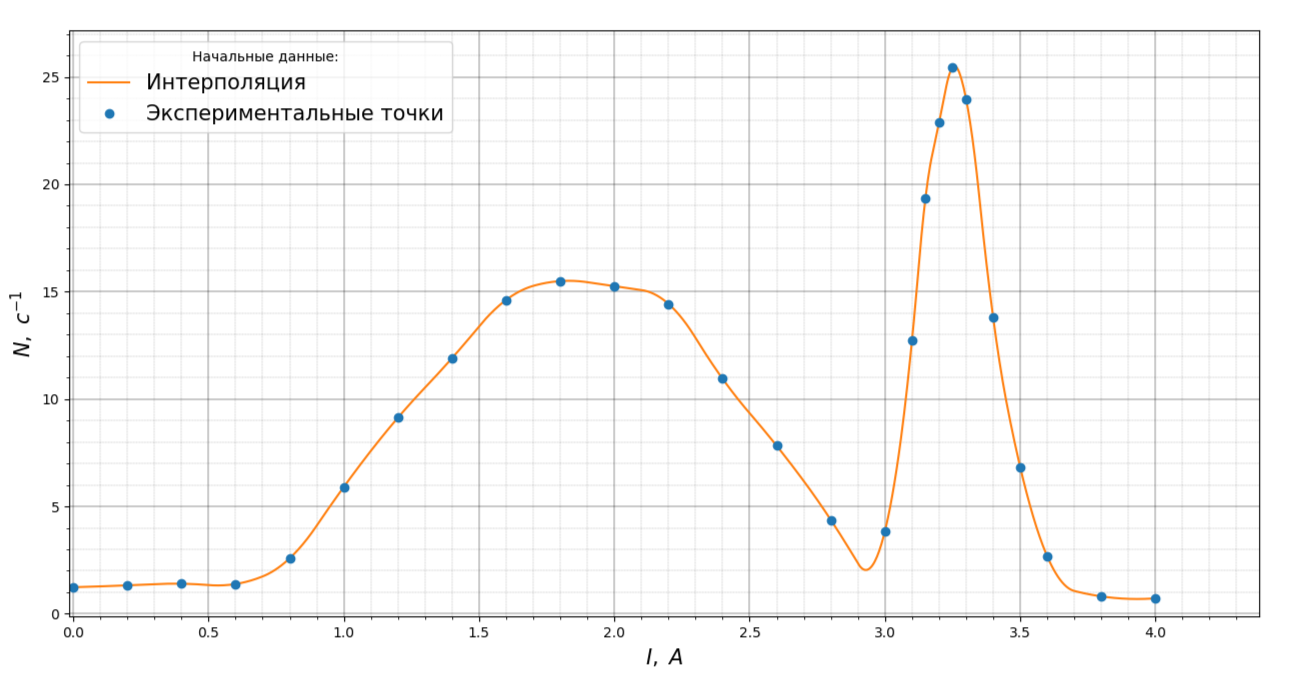
\includegraphics[width=0.9\linewidth]{graph_1}
		\caption{Рис.2, перенесенный в систему построения графиков}
		\label{fig:graph1}
	\end{figure}
	4. Проведем замеры фонового излучения, после нескольких замеров выберем среднее: $N_{\text{ф}}=1.17~c^{-1}$\\
	5. После точного замера $\beta$ распада и получения фонового значения откалибруем результаты по положению конверсионного пика и построим итоговую таблицу.\\
	\begin{table}[H]
		\centering
		\begin{tabular}{|c|c|c|c|c|}
			\hline
			$I$, A & $N-N_{\text{ф}},~c^{-1}$    & $p$, кэВ/с & $E$, кэВ & $mkFermi, \cdot 10^{-3}$   \\ \hline
			0    & 0.067   & 0        & 0      & 0.000 \\ \hline
			0.2  & 0.1545  & 62.4     & 3.8    & 2.335 \\ \hline
			0.4  & 0.2295  & 124.8    & 15     & 0.849 \\ \hline
			0.6  & 0.217   & 187.1    & 33.2   & 0.460 \\ \hline
			0.8  & 1.4165  & 249.5    & 57.7   & 0.408 \\ \hline
			1    & 4.7404  & 311.9    & 87.7   & 0.441 \\ \hline
			1.2  & 7.9642  & 374.3    & 122.4  & 0.417 \\ \hline
			1.4  & 10.738  & 436.7    & 161.1  & 0.378 \\ \hline
			1.6  & 13.4495 & 499      & 203.2  & 0.343 \\ \hline
			1.8  & 14.3243 & 561.4    & 248.1  & 0.296 \\ \hline
			2    & 14.087  & 623.8    & 295.4  & 0.251 \\ \hline
			2.2  & 13.2621 & 686.2    & 344.5  & 0.211 \\ \hline
			2.4  & 9.7759  & 748.6    & 395.3  & 0.162 \\ \hline
			2.6  & 6.6521  & 810.9    & 447.5  & 0.121 \\ \hline
			2.8  & 3.2034  & 873.3    & 500.8  & 0.081 \\ \hline
			3    & 2.6781  & 935.7    & 555.1  & 0.069 \\ \hline
			3.1  & 11.5502 & 966.9    & 582.6  & 0.119 \\ \hline
			3.15 & 18.1977 & 982.5    & 596.4  & 0.143 \\ \hline
			3.2  & 21.7019 & 998.1    & 610.3  & 0.152 \\ \hline
			3.25 & 24.2705 & 1013.7   & 624.2  & 0.156 \\ \hline
			3.3  & 22.8085 & 1029.3   & 638.1  & 0.148 \\ \hline
			3.4  & 12.6373 & 1060.4   & 666.1  & 0.108 \\ \hline
			3.5  & 5.6649  & 1091.6   & 694.3  & 0.072 \\ \hline
			3.6  & 1.504   & 1122.8   & 722.6  & 0.043 \\ \hline
			3.8  & -0.36   & 1185.2   & 779.7  & 0.022 \\ \hline
			4    & -0.45   & 1247.6   & 837.2  & 0.019 \\ \hline
		\end{tabular}
	\caption{Результаты замеров}
	\end{table}
	\begin{center}
		Где: $mkFermi=\frac{\sqrt{N}}{p^{3/2}}$. Используя $mkFermi$ построим график и аппроксимируя его линейную часть найдем пересечение с осью x\\
	\end{center}
	\newpage
	6. Аппроксимируя линейную часть получим: $y=kx+b$, где $k = -0.001$, $b = 0.521$, погрешность аппроксимации не приводится так является несущественной в сравнении с погрешностью счетчика (погрешность определение коэффициентов: $\Delta k \approx 10^{-5}$, $\Delta b \approx 10^{-3}$ - это говорит об удачной аппроксимации)
	\begin{figure}[H]
		\centering
		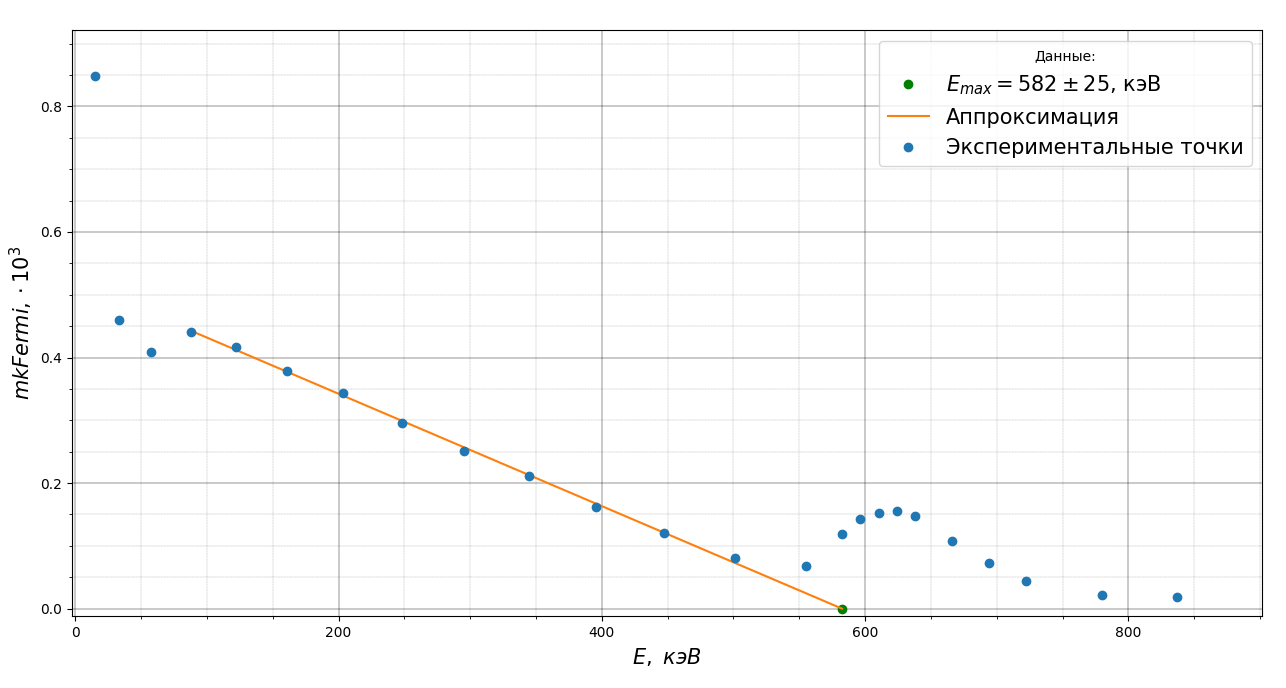
\includegraphics[width=0.9\linewidth]{graph_2}
		\caption{Поиск $E_{max}$}
		\label{fig:graph2}
	\end{figure}
	\begin{center}
	\textbf{	Определили:} $E_{max} = 582 \pm 25~\text{кэВ}$
	\end{center}
	\section{Обсуждение результатов}
	1. В работе пронаблюдали $\beta$ распад $^{137}$Cs, изучили зависимость вероятности вылета частицы с определенной  энергией, экспериментально наблюдали конверсионный пик.\\
	2. Определили максимальную энергию $\beta$ частиц: $E_{max}^{\text{эксп.}} = 582 \pm 25~\text{кэВ}$, $E_{max}^{\text{теор.}} = 634~\text{кэВ}$. В пределах удвоенной погрешности мы попадаем в желаемое значение. Так как результат зависит от множества факторов, данную оценку можно считать верной.\\
	\begin{thebibliography}{9}
		\bibitem{max} \emph{Лабораторный практикум по общей физике. В 3 томах. Том 3. Квантовая физика: учебное пособие} под ред. Ю. М. Ципенюка
	\end{thebibliography}
	
\end{document}